\chapter{Catálise organometálica: etapas elementares e ciclos}\label{ch:b2:catalytic-cycles}

Alguns miligramas de um sal de paládio conseguem unir dois anéis \omterm{def:b2:huckel:aromatic}{aromáticos} em
um balão que contém quilogramas de reagentes: o mesmo átomo metálico faz o
trabalho milhares de vezes, voltando a seu estado inicial após cada
passagem. Como ele o faz é contado por um \omterm{def:b2:catalytic-cycles:cycle}{ciclo catalítico}, uma sequência
fechada de um punhado de etapas elementares. Há apenas alguns tipos de etapa,
e cada um muda de modo fixo o estado de oxidação, a contagem de elétrons e o
número de ligantes do metal. Com a contagem de elétrons do
\cref{ch:b2:coordination-complexes}, um ciclo pode ser lido, verificado e, às
vezes, previsto.

\begin{recall}
\Cref{ch:b2:coordination-complexes}: estado de oxidação, $d^n$, \omterm{def:b2:coordination-complexes:electron-count}{contagem de
elétrons de valência}, \omterm{def:b2:coordination-complexes:electron-count}{regra dos 18 elétrons}, \omterm{def:b2:coordination-complexes:hapticity}{hapticidade}.
\Cref{ch:b2:ligand-field}: ligantes $\pi$-aceptores e \omterm{def:b2:ligand-field:pi-ligands}{retrodoação}. O volume do
1.º ano: catalisador, catálise homogênea, etapa elementar, etapa determinante
da velocidade, composto organometálico, número de oxidação.
\end{recall}

\begin{omfigure}
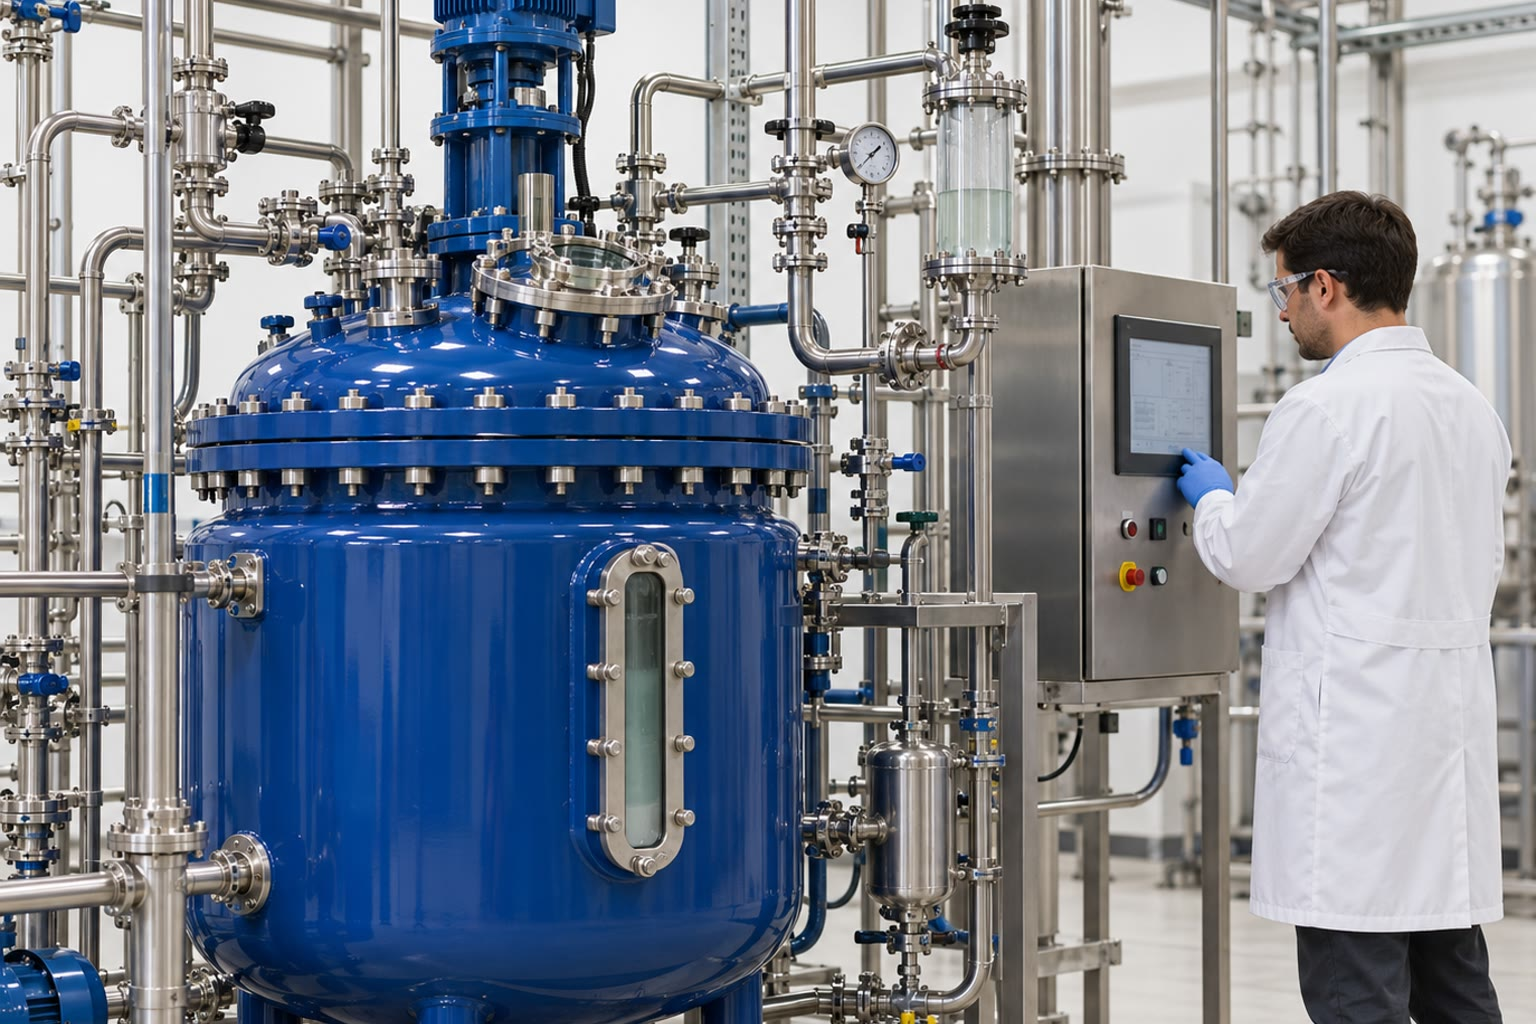
\includegraphics[width=0.62\linewidth]{images/book3/ai/b2-20-pilot-plant.jpg}

{\small Uma planta piloto de química de processos: um reator de aço revestido de
vidro, onde um acoplamento catalisado é ampliado a partir do balão antes da
produção.}
\end{omfigure}

\section{A linguagem dos complexos organometálicos}

Os complexos organometálicos são contados como no \cref{met:b2:coordination-complexes:electron-count},
com alguns ligantes a mais: um hidreto \ce{H-} e um ânion alquila ou arila
\ce{R-} cedem dois elétrons cada um e contam $-1$ no estado de oxidação; \ce{CO},
as fosfinas \ce{PR3} e os $\eta^2$-alcenos cedem dois elétrons e contam 0; um
haleto \ce{X-} cede dois e conta
$-1$.

\begin{definition}[Complexos insaturados]\label{def:b2:catalytic-cycles:unsaturated}
Um \emph{complexo coordenativamente insaturado}\index{complexo coordenativamente insaturado}
tem menos de 18 elétrons de valência (frequentemente 16) e pode ligar mais um
ligante: ele tem um \emph{sítio vacante}\index{sitio vacante@sítio vacante}, uma posição de sua \omterm{def:b2:coordination-complexes:coordination-sphere}{esfera
de coordenação} livre para receber um doador de dois elétrons.
\end{definition}

Os complexos $d^8$ quadrados planos de ródio(I), irídio(I), paládio(II) e
platina(II) são complexos de 16 elétrons; as bisfosfinas de paládio(0) \ce{PdL2}
têm 14. Tais complexos são as espécies ativas da maioria dos \omterm{def:b2:catalytic-cycles:cycle}{ciclos
catalíticos}.

\begin{method}[Contar um complexo organometálico]\label{met:b2:catalytic-cycles:count-organometallic}
\begin{enumerate}
  \item Liste os ligantes: aniônicos (\ce{H-}, \ce{R-}, \ce{X-}, \ce{C5H5-}) e neutros
        (\ce{CO}, \ce{PR3}, alcenos, solvente).
  \item Estado de oxidação = carga do complexo $-$ soma das cargas dos ligantes aniônicos.
  \item $n = g -$ estado de oxidação; contagem = $n + 2 \times$(número de doadores de dois elétrons)
        $+$ 6 por $\eta^5$-\ce{C5H5-}.
  \item Número de coordenação = número de posições de ligante ocupadas.
\end{enumerate}
\end{method}

\section{Troca de ligante, adição oxidativa, eliminação redutiva}

\begin{definition}[Troca de ligante]\label{def:b2:catalytic-cycles:ligand-exchange}
Uma \emph{troca de ligante}\index{troca de ligante} é uma etapa elementar na qual um ligante da
\omterm{def:b2:coordination-complexes:coordination-sphere}{esfera de coordenação} é substituído por outro; ela não muda nem o estado de
oxidação nem, no saldo, a contagem de elétrons. Seus mecanismos são estudados
no volume do 3.º ano.
\end{definition}

\begin{definition}[Adição oxidativa e eliminação redutiva]\label{def:b2:catalytic-cycles:oxidative-addition}
Em uma \emph{adição oxidativa}\index{adicao oxidativa@adição oxidativa}, uma molécula A--B se
adiciona a um centro metálico rompendo sua ligação A--B e formando as ligações
M--A e M--B. Uma \emph{eliminação redutiva}\index{eliminacao redutiva@eliminação redutiva} é a
etapa inversa: dois ligantes A e B, cis um em relação ao outro, se unem em
A--B e deixam o metal.
\end{definition}

\begin{proposition}[Contagem de uma adição oxidativa]\label{prop:b2:catalytic-cycles:oa}
Uma \omterm{def:b2:catalytic-cycles:oxidative-addition}{adição oxidativa} eleva de 2 o estado de oxidação do metal, de 2 sua
\omterm{def:b2:coordination-complexes:electron-count}{contagem de elétrons de valência} e de 2 seu número de coordenação; uma
\omterm{def:b2:catalytic-cycles:oxidative-addition}{eliminação redutiva} diminui cada um de 2.
\end{proposition}

\begin{proof}
Uma vez ligados, A e B são contados como ânions (\ce{H-}, \ce{R-}, \ce{X-}):
dois novos ligantes aniônicos elevam o estado de oxidação de 2 e diminuem $n$
de 2; eles cedem dois pares, $+4$ elétrons; a contagem muda de $-2 + 4 = +2$.
Duas posições passam a ser ocupadas. A etapa inversa reverte cada mudança.
\end{proof}

\begin{example}[O complexo de Vaska]\label{ex:b2:catalytic-cycles:vaska}
\ce{[IrCl(CO)(PPh3)2]}, quadrado plano: irídio(I), $d^8$, 16 elétrons, tetracoordenado.
Ele adiciona di-hidrogênio: \ce{[IrH2Cl(CO)(PPh3)2]}, irídio(III), $d^6$, 18 elétrons,
octaédrico, com os dois hidretos em cis.
\end{example}

\section{Inserção, eliminação, transmetalação}

\begin{definition}[Inserção e eliminação de hidreto $\beta$]\label{def:b2:catalytic-cycles:insertion}
Em uma \emph{inserção migratória}\index{insercao migratoria@inserção migratória}, um ligante insaturado
(alceno, \ce{CO}) ligado ao metal se insere em uma ligação M--H ou M--C cis: \ce{M-H} e
um alceno dão uma alquila \ce{M-CH2-CH2-H}; \ce{M-R} e \ce{CO} dão uma acila \ce{M-C(=O)R}.
Uma \emph{eliminação de hidreto $\beta$}\index{eliminacao de hidreto beta@eliminação de hidreto $\beta$}
é o inverso de uma inserção de alceno: um hidrogênio do carbono $\beta$ em
relação ao metal passa para o metal, liberando um alceno.
\end{definition}

\begin{proposition}[Contagem de uma inserção]\label{prop:b2:catalytic-cycles:insertion}
Uma \omterm{def:b2:catalytic-cycles:insertion}{inserção migratória} conserva o estado de oxidação e diminui de 2 a
contagem de elétrons (uma posição de ligante é liberada); uma eliminação de
hidreto $\beta$ eleva a contagem de 2.
\end{proposition}

\begin{proof}
Antes: \ce{H-} (ou \ce{R-}, aniônico) e o alceno (neutro), dois ligantes, quatro
elétrons. Depois: uma alquila (aniônica), dois elétrons. A carga aniônica não
muda: mesmo estado de oxidação; perdem-se dois elétrons e uma posição.
\end{proof}

\begin{proposition}[Condições da eliminação de hidreto $\beta$]\label{prop:b2:catalytic-cycles:beta-h}
Uma alquila metálica sofre eliminação de hidreto $\beta$ somente se a alquila
tem um hidrogênio em seu carbono $\beta$ e o metal tem um \omterm{def:b2:catalytic-cycles:unsaturated}{sítio vacante} cis em
relação à alquila.
\end{proposition}

\begin{proof}[Raciocínio]
A etapa passa por um arranjo de quatro membros M--C$_\alpha$--C$_\beta$--H no qual
o hidrogênio alcança o metal: ela precisa desse hidrogênio e de uma posição
vazia ao lado da alquila para recebê-lo. Os grupos metila, benzila,
neopentila e arila, que não têm hidrogênio $\beta$ capaz de alcançar o metal,
são estáveis em relação a ela.
\end{proof}

\begin{definition}[Transmetalação]\label{def:b2:catalytic-cycles:transmetalation}
Uma \emph{transmetalação}\index{transmetalacao@transmetalação} transfere um grupo orgânico de
um metal (ou metaloide: boro, zinco, estanho) para outro, em geral em troca de
um haleto.
\end{definition}

\begin{omfigure}
\begin{tikzpicture}[font=\small, >={Stealth}]
  \tikzset{omstepar/.style={->, thick}}
  \foreach \y/\l/\r/\top/\bot/\rev in {
      0/{$\mathrm{L}_n\mathrm{M}$}/{$\mathrm{L}_n\mathrm{M(A)(B)}$}/{+ A--B}/{adição oxidativa}/{eliminação redutiva},
      -1.5/{$\mathrm{L}_n\mathrm{M(H)(CH_2{=}CH_2)}$}/{$\mathrm{L}_n\mathrm{M{-}CH_2CH_3}$}/{}/{inserção migratória}/{eliminação de hidreto $\beta$},
      -3.0/{$\mathrm{L}_n\mathrm{M(X)(R)}$}/{$\mathrm{L}_n\mathrm{M(R)(R')}$}/{+ R$'$--[B], $-$ X--[B]}/{transmetalação}/{},
      -4.5/{$\mathrm{L}_n\mathrm{M(X)}$}/{$\mathrm{L}_n\mathrm{M(X)(L')}$}/{+ L$'$}/{troca ou ligação de ligante}/{}} {
    \node[cyclenode, anchor=east] (l) at (0,\y) {\l};
    \node[cyclenode, anchor=west] (r) at (5.2,\y) {\r};
    \draw[omstepar] ($(l.east)+(0.1,0.08)$) -- ($(r.west)+(-0.1,0.08)$) node[midway, above, font=\scriptsize] {\top};
    \node[font=\scriptsize, anchor=north] at (2.6,\y-0.02) {\bot};
    \node[font=\scriptsize, black!55, anchor=west] at (5.2,\y-0.5) {\rev};
  }
\end{tikzpicture}

{\small As etapas elementares da catálise organometálica. \omterm{def:b2:catalytic-cycles:oxidative-addition}{Adição oxidativa}:
estado de oxidação, contagem e número de coordenação $+2$; \omterm{def:b2:catalytic-cycles:oxidative-addition}{eliminação
redutiva}: $-2$. \omterm{def:b2:catalytic-cycles:insertion}{Inserção migratória}: contagem $-2$, estado de oxidação
inalterado; eliminação de hidreto $\beta$: o inverso. \omterm{def:b2:catalytic-cycles:transmetalation}{Transmetalação}: um grupo
orgânico passa para o metal a partir do boro, do zinco ou do estanho.}
\end{omfigure}

\section{Ler um ciclo catalítico}

\begin{definition}[Ciclo catalítico]\label{def:b2:catalytic-cycles:cycle}
Um \emph{ciclo catalítico}\index{ciclo catalitico@ciclo catalítico} é uma sequência fechada de etapas
elementares que consome os reagentes, libera os produtos e regenera seu
primeiro complexo. O composto adicionado à reação, que se transforma no
primeiro complexo do ciclo, é o \emph{pré-catalisador}\index{pre-catalisador@pré-catalisador}. O
\emph{número de rotação}\index{numero de rotacao@número de rotação} (TON) é a quantidade de produto
formada por quantidade de catalisador; a \emph{frequência de
rotação}\index{frequencia de rotacao@frequência de rotação} (TOF) é o número de rotação por unidade de tempo.
\end{definition}

\begin{proposition}[A equação global]\label{prop:b2:catalytic-cycles:cycle-sum}
A soma das etapas de um \omterm{def:b2:catalytic-cycles:cycle}{ciclo catalítico} é a equação da reação catalisada:
cada complexo metálico aparece uma vez como produto e uma vez como reagente, e
se cancela.
\end{proposition}

\begin{proof}
Sendo o ciclo fechado, cada intermediário é formado por uma etapa e consumido
pela seguinte; somando as etapas, essas espécies aparecem dos dois lados e se
cancelam. Restam as espécies que entram de fora (reagentes) e que saem
(produtos).
\end{proof}

\begin{method}[Ler um ciclo]\label{met:b2:catalytic-cycles:read-cycle}
\begin{enumerate}
  \item Para cada complexo, calcule o estado de oxidação, a contagem de
        elétrons e o número de coordenação.
  \item Dê nome a cada etapa a partir das mudanças ($+2/+2/+2$: \omterm{def:b2:catalytic-cycles:oxidative-addition}{adição
        oxidativa}; contagem $-2$ a estado de oxidação constante: inserção; e
        assim por diante).
  \item Verifique que nenhum complexo ultrapassa 18 elétrons e que uma etapa
        que exige um \omterm{def:b2:catalytic-cycles:unsaturated}{sítio vacante} parte de um complexo insaturado.
  \item Some as etapas: a soma deve ser a equação global.
\end{enumerate}
\end{method}

\begin{omfigure}
\begin{tikzpicture}[font=\small, >={Stealth}]
  \node[cyclenode] (n1) at (90:2.3) {\ce{[RhCl(PPh3)2]}\\ Rh(I), 14 e};
  \node[cyclenode] (n2) at (0:3.4) {\ce{[RhH2Cl(PPh3)2]}\\ Rh(III), 16 e};
  \node[cyclenode] (n3) at (270:2.3) {\ce{[RhH2Cl(PPh3)2(RCH=CH2)]}\\ Rh(III), 18 e};
  \node[cyclenode] (n4) at (180:3.4) {\ce{[RhH(CH2CH2R)Cl(PPh3)2]}\\ Rh(III), 16 e};
  \draw[cyclearc] (n1) to[bend left=20] node[cyclelabel, below left] {adição\\ oxidativa} (n2);
  \draw[cyclearc] (n2) to[bend left=20] node[cyclelabel, left=12pt] {ligação\\ do alceno} (n3);
  \draw[cyclearc] (n3) to[bend left=20] node[cyclelabel, above right] {inserção\\ migratória} (n4);
  \draw[cyclearc] (n4) to[bend left=20] node[cyclelabel, below right] {eliminação\\ redutiva} (n1);
  \draw[cyclein] (4.6,2.3) node[right] {\ce{H2}} -- (2.6,1.75);
  \draw[cyclein] (4.6,-2.3) node[right] {alceno} -- (2.6,-1.75);
  \draw[cycleout] (-2.6,1.75) -- (-4.6,2.3) node[left] {alcano};
  \node[font=\tiny, align=center, black!60] at (0,-0.05) {pré-catalisador\\ \ce{[RhCl(PPh3)3]}\\ perde um \ce{PPh3}};
\end{tikzpicture}

{\small A hidrogenação de um alceno com o catalisador de Wilkinson, simplificada
(trocas de fosfina e de solvente omitidas). As quatro etapas somam
$\ce{RCH=CH2 + H2 -> RCH2CH3}$; os complexos de ródio se cancelam.}
\end{omfigure}

\begin{omfigure}
\begin{tikzpicture}[font=\small, >={Stealth}]
  \node[cyclenode] (s1) at (90:2.3) {\ce{PdL2}\\ Pd(0), 14 e};
  \node[cyclenode] (s2) at (0:3.4) {\ce{[ArPd(Br)L2]}\\ Pd(II), 16 e};
  \node[cyclenode] (s3) at (270:2.3) {$[\mathrm{ArPd(Ar')L_2}]$\\ Pd(II), 16 e};
  \draw[cyclearc] (s1) to[bend left=25] node[cyclelabel, below left] {adição\\ oxidativa} (s2);
  \draw[cyclearc] (s2) to[bend left=25] node[cyclelabel, above left] {transmetalação} (s3);
  \draw[cyclearc] (s3) to[bend left=35] node[cyclelabel, right] {eliminação\\ redutiva} (s1);
  \draw[cyclein] (4.8,2.2) node[right] {\ce{Ar-Br}} -- (2.6,1.6);
  \draw[cyclein] (5.4,-0.9) node[right, align=left] {$\mathrm{Ar'B(OH)_2}$\\ + base} -- (3.3,-1.2);
  \draw[cycleout] (2.3,-2.0) -- (4.4,-2.9) node[right] {\ce{Br-}, \ce{B(OH)3}};
  \draw[cycleout] (-1.75,-0.4) -- (-4.2,-0.4) node[left] {$\mathrm{Ar{-}Ar'}$};
\end{tikzpicture}

{\small O acoplamento de Suzuki, simplificado. O paládio(0) adiciona o brometo de
arila; a base transforma o ácido borônico em borato, que transfere seu grupo
arila ao paládio; as duas arilas, em cis, são eliminadas como a biarila,
regenerando o paládio(0).}
\end{omfigure}

Na reação de Heck, o complexo arila--paládio formado por \omterm{def:b2:catalytic-cycles:oxidative-addition}{adição oxidativa} liga
um alceno em vez de um borato; a \omterm{def:b2:catalytic-cycles:insertion}{inserção migratória} coloca a arila no alceno,
e uma eliminação de hidreto $\beta$ libera o alceno substituído (em geral o
isômero trans) e um hidreto de paládio, do qual uma base retira \ce{HBr} para
regenerar o paládio(0).

A hidroformilação, a adição de \ce{H2} e de \ce{CO} a um alceno para dar um
aldeído, ocorre sobre hidretos de cobalto ou de ródio por inserção do alceno,
inserção de \ce{CO} na ligação metal--alquila, \omterm{def:b2:catalytic-cycles:oxidative-addition}{adição oxidativa} de \ce{H2} e
\omterm{def:b2:catalytic-cycles:oxidative-addition}{eliminação redutiva} do aldeído. O sentido da primeira inserção decide o
produto: o metal no carbono terminal dá o aldeído linear; no carbono interno,
o ramificado; fosfinas volumosas favorecem o produto linear.

\begin{history}[Os acoplamentos cruzados]
\begin{minipage}[t]{0.36\linewidth}
\vspace{0pt}
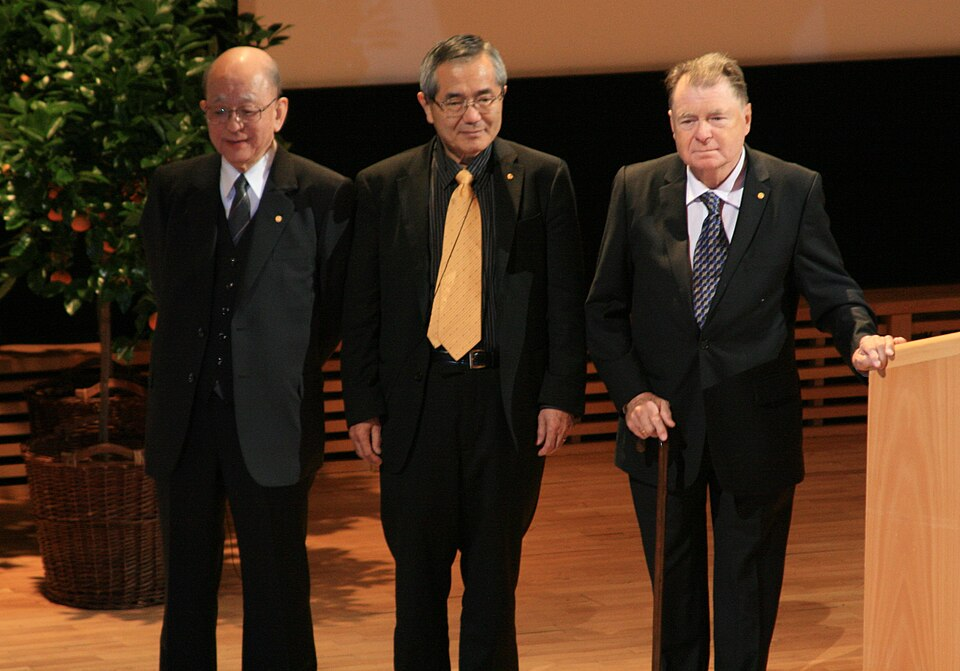
\includegraphics[width=\linewidth]{images/book3/nobel-2010.jpg}
\end{minipage}\hfill
\begin{minipage}[t]{0.6\linewidth}
\vspace{0pt}
Os acoplamentos catalisados por paládio de haletos de arila e de vinila com
alcenos (Richard Heck, a partir de 1968), com organozíncicos (Ei-ichi Negishi,
1977) e com compostos organoborados (Akira Suzuki, 1979) tornaram rotineira a
união de dois esqueletos carbônicos; eles estão hoje entre as reações mais
usadas na fabricação de medicamentos e de materiais. O Prêmio Nobel de Química
foi concedido aos três em 2010. (Fotografia: Suzuki, Negishi e Heck, da
esquerda para a direita, 2010; BloodIce, CC BY-SA 4.0, Wikimedia Commons.)
\end{minipage}
\end{history}

\begin{proposition}[Rotação]\label{prop:b2:catalytic-cycles:tof}
Sendo $n_P$ a quantidade de produto formada em um tempo $t$ por uma quantidade
$n_{\text{cat}}$ de catalisador,
$\mathrm{TON} = n_P/n_{\text{cat}}$, e a \omterm{def:b2:catalytic-cycles:cycle}{frequência de rotação} média é $\mathrm{TOF} =
\mathrm{TON}/t$.
\end{proposition}

\begin{proof}
Cada volta do ciclo produz uma molécula de produto por átomo metálico; o número
de voltas dadas em média por cada átomo é $n_P/n_{\text{cat}}$, e a velocidade
de rotação é esse número por unidade de tempo.
\end{proof}

\begin{safety}{\ghs[5mm]{GHS05}\,\ghs[5mm]{GHS07}\,\ghs[5mm]{GHS09}}
O etanoato de paládio(II) é corrosivo para os olhos e tóxico para a vida
aquática; a trifenilfosfina é nociva e sensibilizante. Eles são pesados na
capela, e os resíduos de paládio são recolhidos para recuperação, nunca
jogados na pia.
% ledger: ghs:Pd-acetate, ghs:PPh3, ghs:phenylboronic-acid, ghs:4-bromotoluene
\end{safety}

\section{Exercícios}

\begin{exercise}[$\star$]\label{exo:b2:catalytic-cycles:1}
Dê o estado de oxidação, o $d^n$ e a contagem de elétrons do complexo de Vaska
\ce{[IrCl(CO)(PPh3)2]} antes e depois de ele adicionar \ce{H2}.
\end{exercise}

\begin{exercise}[$\star$]\label{exo:b2:catalytic-cycles:2}
Dê o nome da etapa: \ce{[PtCl2(CH3)2(PR3)2] -> [PtCl2(PR3)2] + C2H6}; \ce{[Pd(Ph)Br(PR3)2] +
CH2=CH2 -> [Pd(CH2CH2Ph)Br(PR3)] + PR3}.
\end{exercise}

\begin{exercise}[$\star$]\label{exo:b2:catalytic-cycles:3}
Uma reação usa \qty{0.020}{mmol} de catalisador e dá \qty{15.0}{mmol} de produto em
\qty{3.0}{h}. Calcule o TON e o TOF médio.
\end{exercise}

\begin{exercise}[$\star$]\label{exo:b2:catalytic-cycles:4}
Some as três etapas do ciclo de Suzuki e verifique que o paládio se cancela.
\end{exercise}

\begin{exercise}[$\star\star$]\label{exo:b2:catalytic-cycles:5}
Quais destes complexos alquila de paládio podem sofrer eliminação de hidreto $\beta$:
\ce{Pd-CH3}, \ce{Pd-CH2CH3}, \ce{Pd-CH2C(CH3)3}, \ce{Pd-CH2Ph}, \ce{Pd-CH(CH3)2}?
\end{exercise}

\begin{exercise}[$\star\star$]\label{exo:b2:catalytic-cycles:6}
Preveja o produto da reação de Heck do iodobenzeno com o propenoato de metila,
e sua geometria.
\end{exercise}

\begin{exercise}[$\star\star$]\label{exo:b2:catalytic-cycles:7}
Escreva os aldeídos linear e ramificado formados pela hidroformilação do
propeno e explique qual inserção leva a cada um.
\end{exercise}

\begin{exercise}[$\star\star$]\label{exo:b2:catalytic-cycles:8}
Por que o \ce{[RhCl(PPh3)3]} só pode adicionar \ce{H2} depois de perder uma
fosfina, enquanto o \ce{[RhCl(PPh3)2]} o adiciona de imediato?
\end{exercise}

\begin{exercise}[$\star\star$]\label{exo:b2:catalytic-cycles:9}
No acoplamento de Suzuki, por que é necessária uma base, e o que ela faz com o ácido borônico?
\end{exercise}

\begin{exercise}[$\star\star\star$]\label{exo:b2:catalytic-cycles:10}
Um ciclo proposto para a hidrogenação de um alceno sobre um complexo $d^8$ \ce{ML3X} (16 e)
começa pela ligação do alceno, dando um complexo de 20 elétrons, e depois pela
\omterm{def:b2:catalytic-cycles:oxidative-addition}{adição oxidativa} de \ce{H2}. Encontre o erro e corrija a ordem.
\end{exercise}

\begin{exercise}[$\star\star\star$]\label{exo:b2:catalytic-cycles:11}
A quantidade de produto de uma reação catalisada cresce segundo $n_P(t) = n_{\max}(1 - \mathrm e^{-t/\tau})$
com $n_{\max} = \qty{10.0}{mmol}$, $\tau = \qty{40}{min}$ e \qty{0.010}{mmol} de
catalisador (dados do exercício). Calcule o TOF inicial e o TON final.
\end{exercise}

\begin{exercise}[$\star\star\star$]\label{exo:b2:catalytic-cycles:12}
Proponha um acoplamento cruzado para preparar o 4-metoxibifenila, escolhendo o
haleto e o ácido borônico, e escreva o ciclo.
\end{exercise}

\section{Problema: Ler o ciclo de Suzuki}

\begin{problem}[{Problema de fim de semana --- o pré-catalisador e o paládio(0)
ativo, a adição oxidativa, a transmetalação e a eliminação redutiva de um
acoplamento de Suzuki, o rendimento e o número de rotação, e as reações
secundárias}]
\label{pb:b2:catalytic-cycles:1}
Ensaio (dados do exercício): \qty{10.0}{mmol} de 4-bromotolueno, \qty{12.0}{mmol} de
ácido fenilborônico, \qty{20}{mmol} de carbonato de potássio, \qty{0.050}{mmol} de
etanoato de paládio(II) e \qty{0.10}{mmol} de trifenilfosfina em uma mistura de
tolueno, etanol e água, aquecida sob nitrogênio; produto isolado: \qty{1.51}{g}
de 4-metilbifenila. Massas molares (\unit{g/mol}): 4-bromotolueno 171.04, ácido
fenilborônico 121.93, 4-metilbifenila 168.24, etanoato de paládio(II) 224.51.
% ledger: aw:C, aw:H, aw:Br, aw:B, aw:O, aw:Pd

\medskip
\noindent\textbf{Parte I --- O catalisador.}
\begin{enumerate}
  \item Dê o estado de oxidação e o $d^n$ do paládio no etanoato de paládio(II).
  \item No balão, ele é reduzido a \ce{Pd(PPh3)2}. Dê seu estado de oxidação, seu
        $d^n$ e sua contagem de elétrons.
  \item Por que esse complexo é coordenativamente insaturado?
  \item Por que a reação é conduzida sob nitrogênio?
  \item Qual é o papel do excesso de trifenilfosfina?
  \item O etanoato de paládio(II) é o catalisador ou o \omterm{def:b2:catalytic-cycles:cycle}{pré-catalisador}?
\end{enumerate}

\medskip
\noindent\textbf{Parte II --- As etapas.}
\begin{enumerate}[resume]
  \item Escreva a \omterm{def:b2:catalytic-cycles:oxidative-addition}{adição oxidativa} do 4-bromotolueno e conte o produto.
  \item O que o carbonato faz com o ácido fenilborônico?
  \item Escreva a \omterm{def:b2:catalytic-cycles:transmetalation}{transmetalação}.
  \item Por que os dois grupos arila precisam estar em cis antes da etapa seguinte?
  \item Escreva a \omterm{def:b2:catalytic-cycles:oxidative-addition}{eliminação redutiva} e conte a espécie de paládio formada.
  \item Some as três etapas.
\end{enumerate}

\medskip
\noindent\textbf{Parte III --- Rendimento e rotação.}
\begin{enumerate}[resume]
  \item Qual reagente é o limitante?
  \item Calcule a quantidade de produto isolada.
  \item Calcule o rendimento.
  \item Calcule a carga de catalisador em mol~\% em relação ao brometo.
  \item Calcule o \omterm{def:b2:catalytic-cycles:cycle}{número de rotação} do paládio.
  \item O ensaio durou \qty{4.0}{h}. Calcule a \omterm{def:b2:catalytic-cycles:cycle}{frequência de rotação} média por hora.
\end{enumerate}

\medskip
\noindent\textbf{Parte IV --- Reações secundárias.}
\begin{enumerate}[resume]
  \item Encontra-se um pouco de bifenila \ce{Ph-Ph}. Sugira como ela se forma.
  \item Por que aqui não é possível nenhuma eliminação de hidreto $\beta$?
  \item Um cloreto de arila reage muito mais lentamente que o brometo. Qual etapa é afetada?
  \item O que acontece com o paládio no fim da reação, e por que ele é recuperado?
  \item Por que se usa um pequeno excesso de ácido borônico?
  \item Dê o \omterm{def:b2:catalytic-cycles:cycle}{número de rotação} do paládio no ensaio.
\end{enumerate}
\end{problem}
